%\documentclass[11pt]{report}
%\usepackage{siunitx}
%\usepackage{graphicx}
%\usepackage[table,xcdraw]{xcolor}
%\usepackage{csquotes}

%\begin{document}
%\setcounter{chapter}{6}
%\tableofcontents


\newpage
\chapter{Global Discussion}
This chapter presents an overall discussion of this dissertation content, starting from summarising its key findings, understanding the major limitations present in the current work, and pointing to future perspectives of the work developed.



\newpage
\section{Main outcomes of this work}

As seen in the previous chapters, the application of numerical modelling techniques to perform predictions in \acs{BTE} stimulation contexts can be an essential tool to optimize and control the induced effects in \textit{in vitro} cell cultures. Numerical models, using finite-element methods and lumped-element methods (electric circuit analogs) were used to predict \textit{in vitro} microenvironmental conditions produced by developed and reported experimental setups under known inputs. This kind of numerical modelling framework was able to provide precise estimates of the delivered E-Field (Chapters 4, 5, and 6) or fluid flow-induced shear stress (Chapters 3 and 6) in the cell culture region for a specific combination of bioreactor setup and scaffold geometry. Best practices \cite{Klein2022-yj} point out the importance of validating the numerical model predictions with experimental measurable outcomes and confronting them with the corresponding model prediction. This study was performed in Chapter 6 for systems delivering \acs{EF} and fluid flow-induced shear stress. This work was committed to effectively share all developed systems and models under an open-source licensing attribution for scientific purposes, including configuration files for hardware, firmware, software, fabrication blueprints, analyzed data, \acs{CAD} files, and many others required to reconstruct the developed physical setups, stimulation systems, and their corresponding digital models. In this way, this work contributes to fill in the existent gap in the scientific reproducibility and strengthens the need for developing common practices for stimulation protocols and bioreactor \textit{in vitro} cell culture operation for \acs{BTE} and other \acs{TE} areas. It is possible to compare the current version of the developed bioreactor with a list of key features required for a proposed ideal bioreactor system as identified by Ahmed \textit{et al.} \cite{Ahmed2019-uk}. This comparison is available in Table \ref{tabBioreactor}, where we can observe that the current bioreactor development integrates most of the critical features previously identified as essential, and also expands these to include easy and precise reproducibility by designing it specifically to be produced using \acs{3D} printing fuse deposition modelling fabrication. 


\begin{table}[ht]
\caption{Comparison between “must have” features that a new generation of bioreactors should include according to Ahmed \textit{et al.} \cite{Ahmed2019-uk} and current JANUS bioreactor features.}
\bigskip
\scriptsize
\centering
\begin{tabularx}{370px}{l l c} \toprule[0.15em]
\textbf{Features} & \textbf{Advantages} & \textbf{JANUS Bioreactor} \\ \cmidrule(l){1-3}
\rowcolor[HTML]{EEEEEE} 
\textit{Leakproof} & Reduces the risk of contamination and loss of reagents. & {\color[HTML]{38761D} \textbf{TRUE}}  \\
\rowcolor[HTML]{FFFFFF} 
\textit{Optically Transparent} & Allows in situ real-time monitoring. & {\color[HTML]{FF0000} \textbf{FALSE}} \\
\rowcolor[HTML]{EEEEEE} 
\textit{Easy to Assemble} & Less training required, rapid experimental set-up. & {\color[HTML]{38761D} \textbf{TRUE}}  \\
\rowcolor[HTML]{FFFFFF} 
\textit{Ability to monitor} & Provide data on culture conditions such as pH, & \\ 
\textit{microenvironment} & oxygen, carbon dioxide, metabolites. & {\color[HTML]{38761D} \textbf{TRUE}} \\
\rowcolor[HTML]{EEEEEE} 
\textit{Allows use of different flow} & Different flow rates/types are required & \\
\rowcolor[HTML]{EEEEEE} 
\textit{types/rates} & for different cell types/applications. & {\color[HTML]{38761D} \textbf{TRUE}} \\
\rowcolor[HTML]{FFFFFF} 
\textit{Allows easy insertion and} & Allow 3D cell culture and post-analysis. & \\
\textit{retrieval of scaffolds} & & {\color[HTML]{38761D} \textbf{TRUE}} \\ 
\rowcolor[HTML]{EEEEEE} 
\textit{High throughput} & Faster data acquisition. & {\color[HTML]{38761D} \textbf{TRUE}} \\ 
\rowcolor[HTML]{FFFFFF} 
\textit{Flexible configuration} & Modular interconnected systems allow co-culture and & \\
& cell-cell signaling & {\color[HTML]{38761D} \textbf{TRUE}}  \\
\rowcolor[HTML]{EEEEEE} 
\textit{No air bubble formation} & The presence of air bubbles can disrupt the flow rate and  & \\
\rowcolor[HTML]{EEEEEE} 
 & disturb cells. & {\color[HTML]{38761D} \textbf{TRUE}}  \\ \bottomrule[0.15em] 
\end{tabularx}
\label{tabBioreactor}
\end{table}


As shown in Chapter 5, numerical models can also be used to perform meta-analyses of literature-reported setups and protocols. Eight \acs{CCoupled} setups, that were used in twenty studies published between 1978 and 2021, were reproduced and analyzed numerically to observe if the reported \acs{EF} matched the numerical prediction of three different models. It was found that the \acs{EF} was correctly estimated in only 3 out of 8 setups. In 12 out of 20 studies, the overestimation may have led to incorrect assumptions on the effects of stimulation on the observed cellular effects, thus requiring reinterpretation. Numerical models can also be useful to adapt stimulation protocols for different stimulation setups, integrating previously reported results from the literature in recent designs, and additionally, allowing for more reliable comparisons between different experimental outcomes. Methods and results from Chapter 4 for \acs{DCoupled} stimulation setups, regarding experimental protocols and their biologically produced effects can be further refined, by exploring further the experimental characterization of the phenomena involved (electrochemical impedance spectroscopy of the materials involved, electric double layer response, ionic mobility, etc), gathering data that can be introduced into numerical models, contributing to a deeper knowledge of the stimulation phenomena and related biological effects. 

Finally, this work introduced a scaffold structure into the empty cell culture chamber numerical models. The presence of a scaffold in a cell culture, considering its specific geometry and material properties, was shown in Chapters 5 and 6 to have a crucial influence in the generated \acs{EF} and fluid flow-induced shear stress stimulation delivered to the cell culture. The impact of this structure and eventual morphology deviations among the produced scaffolds (when compared to the geometrical ground truth) should be considered in simulation predictions and accounted for as a variability source, often neglected in experimental studies. 




\section{General limitations of this work}

\acs{FEM} was the numerical modelling technique most applied in this research. Recursively applied to different systems/setups geometries and material characteristics, it was essentially reduced to two major sets of equations implemented by COMSOL Multiphysics: one considering the physical phenomena of fluid laminar flow and the other considering electric currents. The considered setup geometries (bioreactors, culture wells, scaffolds) are geometrically simple, however when combined under the same model, require a larger complexity of the mesh to be computed, which had to be adapted for different size scales differing by an order of \num{d6} or higher. This added unprecedented complexity to the model, increasing the computational time required to find a solution, which may originate non-linear and singularity errors, specifically for coarse meshes, limiting the execution of mesh-independent studies. This difficulty was circumvented by considering the finner mesh possible to run on the physical machine available and by selecting a solver with adaptative mesh refinement \cite{Verfuhrt1996-hy}.

Material properties that feed the constructed numerical models were mostly obtained from the literature, an option that induces uncertainty upon the validation of the developed model with a particular setup and cell culture conditions. To decrease this uncertainty, an extensive material characterization should be performed, for example, to determine the response of a particular material to an electric current / electric potential application through experimental techniques, such as impedance spectroscopy, cyclic voltammetry, and chronoamperometry. If this material composes an electrode, its interface with the electrolyte should also be extensively characterized.    

Although this work used well-established electric currents and laminar fluid flow models, other physical/chemical phenomena, not covered by the applied modelling frameworks, may also contribute to the observable biological effects. For example, electrophoresis or dielectrophoresis responses may occur when using electric stimulation signals. These are defined as the motion of suspended particles (including mammalian cells) caused by polarization effects in inhomogeneous electric fields. All particles exhibit dielectrophoretic activity in the presence of electric fields \cite{Park2020-lj, Pethig_undated-bv}. However, the strength of the force depends strongly on the medium and particles' electrical properties, on the particles' shape and size, as well as on the frequency of the electric field. Consequently, fields of a particular frequency can manipulate particles with great selectivity. Another limiting assumption is that
the culture medium is typically assumed to be a homogeneous distribution of chemical species, however, external stimulation might originate heterogeneous space regions with a specific concentration of chemical species, that may constitute probable cause for some effects that cannot be directly attributed to the applied \acs{EF} magnitude. Ratchetaxis phenomena, for example, suggest that cell motility can be viewed as a stochastic phenomenon, which can be biased by various types of local cues, leading to directional migration, which includes electric and shear stress interactions \cite{Zhao2011-wy}, and also cues from cell attachment surface topology, chemical gradients, mechanical stiffness, among others \cite{Caballero2015-cs, Pieuchot2018-kl}. 




\section{Future work}
The evolution of this work can be expected to occur in each of the three main axes addressed in this work: experimental setup design and fabrication; correspondent numerical model construction and validation; and new cell culture stimulation protocols. 

Bioreactor design represents a continuous and laborious effort. Our JANUS design represents the end of a work journey, but not the end of the development line. Future versions should include an improved set of optical sensors (to avoid electromagnetic interference from the electrical stimulation) and become completely watertight and autoclave sterilizable immediately after the \acs{3D} printed process, without requiring further coating applications. Once specifically optimized for that purpose \acs{3D} printing processes have shown to be capable of producing parts without deformation, made from polymeric materials that endure typical autoclave sterilization processes, like polycarbonate, polystyrene, polyetherketoneketone or polyetherimide. Watertight and sterilizable outcomes could then be achieved with high-performance fuse deposition modelling printers by using large nozzles, closed warm chambers, and high processing temperatures. 

These updates will enable an even more reusable bioreactor capable of sustaining a series of experimental works to characterize a precursor cell response to isolated or combined electrical and mechanical stimuli, an experiment where all protocols could be previously established and refined with validated numerical models for that particular bioreactor design.    

The numerical model's construction needs to evolve to open-source systems, like the FEniCSx project \cite{Logg2012-yy}, ensuring a wide acceptance and utility of the developed models with associated low to no-cost solutions. Life sciences, and in particular \acs{BTE} and \acs{TE} areas would strongly benefit from the adoption of common platforms and systems, to facilitate integration of recent developments into existent workflows. This standardization should also include systematic characterization of the properties of the involved materials (e.g. mechanic, electric, rheologic) to feed the developed models, and subsequent steps of validation and uncertainty quantification. Another challenge to overcome is to unite electric and fluid flow phenomena into the same numerical model, using theoretical frameworks such as particle models (rooted in physical matter interactions), from which possible interplays between different stimulation modalities may be identified.

The developed bioreactor with multimodal capabilities (electric and mechanic stimulation), associated with the methodology of using digital models to define and predict the delivered ranges of stimulation, can be improved by integrating real-time sensor readings into the model inputs, achieving the prospects of becoming a digital twin, by the definition provided by Singh \textit{et al.} \cite{Singh2021-ij}:

 \begin{quotation}
\textit{''A Digital Twin is a dynamic and self-evolving digital/virtual model or simulation of a real-life subject or object (part, machine, process, human, etc.) representing the exact state of its physical twin at any given point of time via exchanging the real-time data as well as keeping the historical data. It is not just the Digital Twin which mimics its physical twin but any changes in the Digital Twin are mimicked by the physical twin too.''}
 \end{quotation}
 
This will allow increasing automation of the cell culture and monitoring of the stimulation protocol. Updating the digital twin continuously to reflect a changing environment can help to continuously adjust stimulation towards an equilibrium state, or even modulate a sequence of cellular events, each one requiring a different set of stimulation parameters. Strong divergences between the experimental readings and model predictions are indicative of the knowledge gap of the underlying phenomena or the presence of an unpredicted effect taking place; Online updates of digital twins can thus conduct to improved perception of the process, contributing decisively to improve all involved parts: model, stimulation protocol, and biological outcomes.    




\section{The future of stimulation numerical modelling in \acs{BTE}}

The future of numerical modelling in \acs{BTE} and \acs{TE} in general is strongly connected to the improvement of control and actuation strategies in active cell cultures \cite{Geris2018-tz}. Bioreactors capable of sustaining high cell numbers and long-term cell cultures are required to achieve viable tissues for patient reimplantation, able to sustain mature and adequate cellular metabolic profile. The required microenvironment is growing in complexity as the envisioned strategy aims to progressively mimic the native \textit{in vivo} conditions. New control and actuation features in bioreactor operation should minimize human intervention, being ideally operated in a sterile environment, closely monitored by an automatic system (e.g. machine learning based) that continuously performs experimental recording, along with the numerical predictions scenarios of the cellular microenvironment evolution for real-time accurate control (feedback-controlled) and actuation over the entire cell culture. It is possible to envision a system as presented in Figure \ref{figFuture}, where a digital twin of the fabricated bioreactor, including all contained scaffold structures, could predict the microscale environment for a combination of macroscale inputs \cite{Cioffi2008-kj, Spencer2013-pg}. This multiscale model requires an adequate methodology to integrate the different scale dependencies \cite{Bhattacharya2021-su}, a methodology that, once successfully implemented, may lead to the prediction of different cell culture scenarios from where specific algorithms can pick the local optimal path to improve an outcome, like cell differentiation. Automatically updating the cellular microenvironment conditions by actuating over macroscale bioreactor inputs, and controlling their microscale effects by comparing their numerical predictions against sensor readings at known points, and/or metabolic products assessment with noninvasive microscopy \cite{Neto2023-gd} may become a game changer in bioreactor operation and in precise application of external stimulation \cite{Zimmermann2023-gm, Konig2022-bs}. 

The future of numerical models in \acs{BTE} will probably be driven by an expansion of the current physics models to progressively include more phenomena and recent biology findings \cite{Moller2021-kr}. This may include models of complex biological behaviors and evolving material properties \cite{Metz2020-vr}, interchained with models to calculate the microenvironment, in a way that they introduce geometry updates to reflect the neotissue formation and its related impact (Figure \ref{figFuture}). Growing tissue is a major issue, since as tissue mass increases, the interconnected pores of the scaffold become more and more obstructed, giving rise to changes in mechanical shear stress and in the electric field stimulation acting on the cells. If the stimulation intensities are not adapted to the growing tissue, it may lead to detrimental effects on the cell culture \cite{Vetsch2015-xz}. Possibilities for neotissue formation modelling could include: cell seeding strategies models \cite{Coy2020-st, Nguyen2018-dq, Taghian2015-hf} cells migration abstraction models \cite{Colombi2021-ow}; cells agent-based models or other theoretical frameworks that account for metabolic and differentiation responses \cite{Lopez2019-qj, Dawson2020-mo}; fluid-structure interaction interface models to account for cell mechanical stimuli transduction \cite{Vaughan2013-gj}; cellular membrane response \cite{Gschwend2020-ep} models and many others. Microenvironmental models on their own could expand to integrate nutrient diffusion patterns, oxygen delivery models, energy fluxes, physical and chemical surface properties, and so forth.

\begin{figure}
\makebox[\textwidth][c]{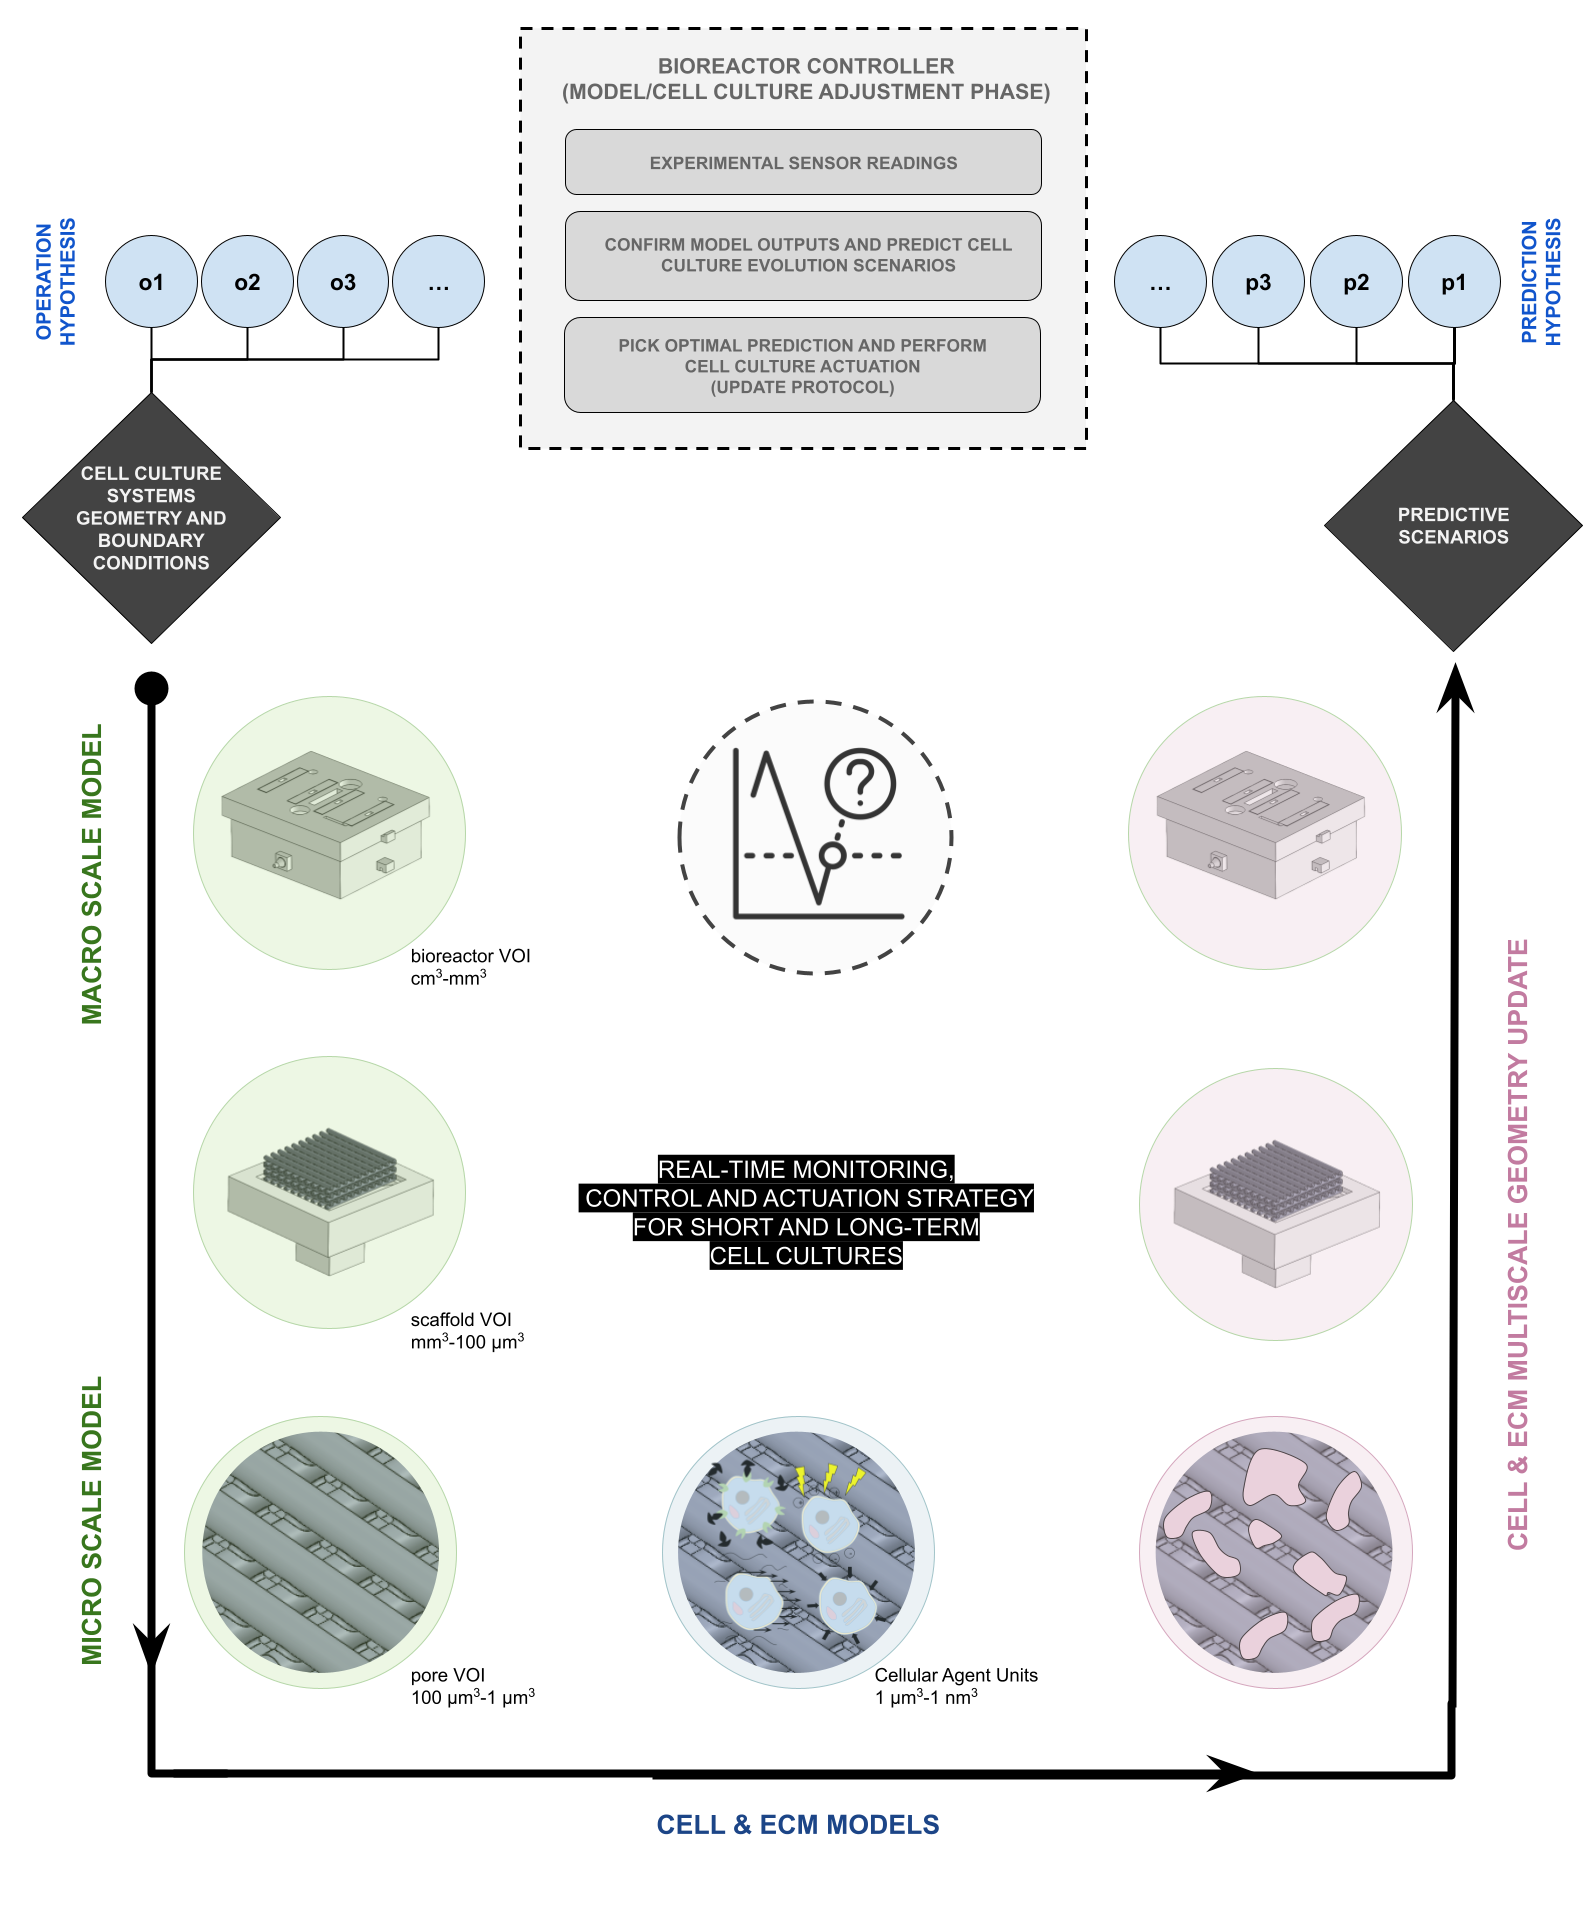
\includegraphics[scale=0.26]{./figures/Figure_7d1}}
\caption{Futuristic concept of the connection between multiscale, multisubject \acs{BTE} / \acs{TE} numerical models and bioreactor monitoring, control, and operation.}
\label{figFuture}
\end{figure}        

The possibility of combining different models, including biology models, will help us to identify the underlying phenomena when comparing the numerical predictions versus the experimental measurements \cite{Geris2018-tz}. Regarding \acs{BTE}, most of the studies so far have focused on mechanics only and neglected the biology \cite{Vetsch2015-xz}. For example, according to the proposed Wolff's Law, bone is deposited and reinforced in areas of greatest stress \cite{Ahn2009-ja}. Despite this law being historically supported from a mechanistic point (by relating physical activity and bone density), a lack of scientific evidence on how this mechanosensory function is performed by bone cells still persists. \textit{In vivo} and \textit{in vitro} numerical modelling of realistic bone conditions, considering strain-generated potentials models (possibly combining bone collagen piezoelectricity and ionic streaming potential) can improve the understanding of how these mechanosensory mechanisms function, while simultaneously assisting experimental setups designs able to recreate the required conditions and protocols to isolate/combine them.

As once stated by P. W. Anderson, a physics Nobel laureate: \enquote{More is Different} \cite{Anderson1972-og}, when referring to the broken symmetry problem, highlighting that the increased hierarchy or specialization of function in a large system, like the ones studied in biology, unexpectedly leads to new rules and processes that arise from the interplay of their simpler parts. Progressively approaching these complex phenomena by bringing different models together may get us one step closer to a new understanding of their underlying reality.  




% VER SE FAZ SENTIDO INCLUIR
%Another interesting experimental observation is made by Rodríguez \textit{et al.} \cite{Fuentes-Rodriguez2022-ey} when placing macroscopic pieces of electric conducting material between immersed parallel plate electrodes. Those, when subjected to the external field polarize throw bipolar induction, generating redox species at the induced poles of opposite charge. The effects observed in these macroscopic metal pieces may be translatable to tissue engineering works when placing conductive scaffolds between electrodes in setups similar to the one applied in this study. Claiming attention to the locally induced effects produced by scaffold material insertion into the stimulation chamber, as predicted previously by our group in a numerical study \cite{Meneses2021-nd}.
%
%Building a clear understanding of DCoupled setups E-Field stimulation and the biophysics of cellular transduction will require a strong electrochemistry characterization of all the materials involved in the electrode/electrolyte interface and in the bulk culture medium region. Several technologies may improve our bioelectrical view of cell behaviour as proposed by \cite{Schofield2020-wz}. Applying currently available bio-electrochemical tools like scanning-ion-conductance (SICM) and scanning-electrochemical-microscopy (SECM) will allow combined mapping of ionic conductivity and redox reactions, respectively, at multiple cell-scale levels, which may unveil the electrical and chemical potential differences across cellular membranes and the electrochemical gradients (ion motive forces) that are effectively being activated by external E-Field stimulation.



%\newpage
%\bibliography{library_c7} 
%\bibliographystyle{plain}
%\end{document}